% !TeX program = xelatex
% 한글 보고서. 본문 10쪽 이내, 참고문헌과 부록은 별도.
\documentclass[a4paper,10pt,twocolumn]{article}
\usepackage{kotex}
\usepackage[margin=18mm,top=20mm,bottom=20mm,columnsep=6mm]{geometry}
\usepackage{amsmath,amssymb}
\usepackage{booktabs,tabularx,array,multirow}
\usepackage{enumitem}
\usepackage{xcolor}
\usepackage{graphicx}
\usepackage[export]{adjustbox}
\usepackage{float}
\usepackage[font=small,labelsep=period]{caption}
\usepackage{tikz}
\usetikzlibrary{arrows.meta,positioning,shadows,calc,backgrounds}
\newfontfamily\figsans{Noto Sans CJK KR}
\usepackage{pgfplots}
\pgfplotsset{compat=1.16}
\usepackage{fancyhdr,lastpage}
\usepackage[unicode,hidelinks]{hyperref}
\usepackage{xurl}
\usepackage{setspace}
\setstretch{1.12}
\setlength{\parindent}{0pt}
\setlength{\parskip}{4pt}
\setlength{\headheight}{16pt}
\setlength{\emergencystretch}{3em}
\renewcommand{\topfraction}{0.85}
\renewcommand{\textfraction}{0.1}
\renewcommand{\floatpagefraction}{0.8}
\renewcommand{\dbltopfraction}{0.85}
\renewcommand{\dblfloatpagefraction}{0.8}
\setcounter{dbltopnumber}{2}
\setlist[itemize]{leftmargin=1.5em,itemsep=1pt,topsep=2pt}
\setlist[enumerate]{leftmargin=1.6em,itemsep=1pt,topsep=2pt}
\renewcommand{\arraystretch}{1.15}
\newcolumntype{Y}{>{\raggedright\arraybackslash}X}
\definecolor{accent}{HTML}{234C70}
\definecolor{light}{HTML}{EFF4F8}
\definecolor{afs}{HTML}{234C70}
\definecolor{rnd}{HTML}{B0BEC5}
\pagestyle{fancy}
\fancyhf{}
\fancyhead[L]{\small Physical AI 작업 수행 검증 및 회귀 테스트 자동화}
\fancyfoot[C]{\small \thepage}
\newcommand{\code}[1]{\texttt{\detokenize{#1}}}
\renewcommand{\refname}{참고문헌}
\captionsetup[table]{name=표}
\captionsetup[figure]{name=그림}
\hypersetup{
  pdftitle={AI 기반 Physical AI 작업 수행 검증 및 회귀 테스트 자동화 기술},
  pdfsubject={행동 피드백 기반 능동 실패 탐색},
  pdfauthor={}
}

\begin{document}

\twocolumn[
% ================================================================== 표지·초록
\begin{center}
  {\LARGE\bfseries AI 기반 Physical AI 작업 수행 검증 및\\[3pt]
  회귀 테스트 자동화 기술\par}
  \vspace{6pt}
  {\large 행동 피드백 기반 능동 실패 탐색: 로봇팔 pick-and-place와 휴머노이드 사례\par}
  \vspace{4pt}
  {\small 2026년 10월}
\end{center}
\begin{center}
\begin{minipage}{0.9\textwidth}
\small
\textbf{요약.}
Physical AI는 물체 배치, 장애물, 작업자 위치 등 3D 환경 변화에 따라 같은 명령에서도
다른 결과를 낸다. 본 과제는 장면 파라미터로부터 시뮬레이션 환경을 자동 생성하고,
이전 실행의 행동 기록을 읽은 LLM이 실패 가능성이 높은 다음 환경을 제안하는
능동 실패 탐색(Active Failure Search, AFS)과, 실행 결과를 판정·보존하여 회귀 테스트로
재사용하는 파이프라인을 구현하였다. LIBERO Panda 로봇팔과 공개 VLA 정책
GR00T~N1.7의 pick-and-place 실험에서 AFS는 동일 예산(12회)으로 실패 발견율
\textbf{58.3\%}를 기록해 Random(16.7\%) 대비 \textbf{3.5배}의 실패를 발견했다.
G1 휴머노이드의 동적 사람 횡단 환경에서도 AFS는 40\%, Random은 0\%였다.
전체 실험에서 초기 정의한 실패 유형 6종 중 \textbf{4종}(충돌, 장애물 간섭, 목표 위치 점유,
작업자 안전 위험)과 도달 불가 후보 1종을 자동 발견하여 세 가지 목표 지표를 모두 달성하였다.
\end{minipage}
\end{center}
\vspace{5mm}]

% ================================================================== 1
\section{서론}

\subsection*{배경과 문제}
제조·물류 현장에 로봇팔, AMR, 시각-언어-행동(VLA) 모델~\cite{rt2} 기반 Physical AI의 도입이 늘고 있다. 이들은 실제 공간에서
행동하므로 소프트웨어 정확도만으로는 품질을 보장할 수 없고, 물체 위치 변화나 장애물 추가,
작업자 접근에 따라 현장에서 실패할 수 있다. 현재의 검증은 사람이 예상 가능한 케이스를
수작업으로 정의하거나 실제 장비에서 제한적으로 반복하는 방식에 의존한다. 이 방식은
테스트 작성에 시간이 들고, 충돌·안전 위험이 있으며, 드문 실패나 PASS/FAIL 경계 조건을
체계적으로 찾기 어렵다. 현장 배치가 바뀔 때마다 테스트를 다시 작성해야 하는 것도 문제다.

\subsection*{목표 지표}
과제의 평가 지표와 목표는 표~\ref{tab:metric}과 같다. 세 지표 모두 같은 시험 예산에서 Random 탐색과 비교한다.
\begin{table*}[!t]
\centering\small
\caption{과제 평가 지표와 목표}\label{tab:metric}
\begin{tabularx}{\textwidth}{@{}p{38mm}Yp{40mm}@{}}
\toprule
지표 & 정의 & 목표 \\
\midrule
실패 발견율 (FDR) & 유효 테스트 중 작업 실패를 발견한 비율, $N_{\mathrm{FAIL}}/N_{\mathrm{VALID}}$ & 30\% 이상 \\
실패 탐색 성능 향상 (Gain) & 동일 테스트 예산에서 Random 대비 실패 발견 향상 & 20\% 이상 \\
실패 유형 다양성 & 사전 정의한 주요 실패 유형 6종 중 자동 발견한 유형 수 & 6종 중 4종 이상 \\
\bottomrule
\end{tabularx}
\end{table*}

\subsection*{기여}
\begin{enumerate}
\item 장면 파라미터로부터 3D 장면 그래프, 이동 지도, 물리 시뮬레이션 모델을 일관되게 생성하고 실행 전에 유효성을 검사하는 환경 생성기.
\item 이전 실행의 행동, 로봇 기능 호출 결과, 측정값을 근거로 다음 테스트 환경을 제안하는 LLM 기반 AFS와 후보 검증기.
\item 실행 유효성, 목표 달성, 실패 유형을 단계적으로 판정하는 평가기와 6종/12종 실패 분류 체계.
\item 로봇팔(VLA)과 휴머노이드(LLM Agent) 두 플랫폼에서 Random 대비 AFS의 실패 탐색 효율을 검증.
\item 발견한 실패·성공 사례를 다시 실행하여 이전 결과와 비교하는 회귀 테스트 실행기.
\end{enumerate}

% ================================================================== 2
\section{관련 연구}
자율 시스템의 안전 검증은 시스템을 블랙박스로 두고 실패를 유발하는 입력을 탐색하는
falsification 문제로 다뤄져 왔다. Corso 등은 최적화, 경로 계획, 강화학습, 중요도 샘플링 기반
블랙박스 안전 검증 기법을 정리하였고~\cite{corso}, Adaptive Stress Testing은 강화학습으로 가장 가능성
높은 실패 경로를 찾는다~\cite{ast}. 본 과제는 탐색기로 LLM을 사용하여, 수치 신호뿐 아니라 행동 기록과
로봇의 기능 호출 결과 같은 비정형 관측을 다음 시험 설계의 근거로 활용한다는 점이 다르다.

로봇 조작 분야에서는 robosuite~\cite{robosuite} 기반의 LIBERO가 언어 조건 조작 과제의 표준 벤치마크를 제공하며~\cite{libero},
GR00T~N1은 범용 휴머노이드·조작 VLA 기반 모델이다~\cite{groot}. 물리 시뮬레이션에는
MuJoCo~\cite{mujoco}를 사용하였다. 3D Scene Graph는 객체와 공간 관계를 계층 그래프로 표현하는
방식으로~\cite{sg}, 본 과제에서 테스트 공간을 구조화하는 입력 표현으로 사용한다.
본 보고서에 나오는 도구와 용어는 부록 F에 정리하였다.

% ================================================================== 3
\section{시스템 구성}

\begin{figure*}[!t]
\centering
\definecolor{c1}{HTML}{4F46E5}\definecolor{c1l}{HTML}{EEF0FD}
\definecolor{c2}{HTML}{0F8B7E}\definecolor{c2l}{HTML}{E8F6F4}
\definecolor{c3}{HTML}{C2620A}\definecolor{c3l}{HTML}{FDF3E7}
\definecolor{cg}{HTML}{475569}\definecolor{cgl}{HTML}{F1F5F9}
\begin{tikzpicture}[x=1mm,y=1mm,font=\figsans\footnotesize,
  panel/.style={rounded corners=2.5mm,line width=0.6pt},
  card/.style={rounded corners=1.5mm,fill=white,draw=#1!45,line width=0.5pt,
    minimum width=36mm,minimum height=13mm,align=center,
    drop shadow={opacity=0.12,shadow xshift=0.5mm,shadow yshift=-0.6mm}},
  title/.style={font=\figsans\footnotesize\bfseries},
  sub/.style={font=\figsans\scriptsize,text=cg},
  badge/.style={circle,fill=#1,text=white,inner sep=0pt,minimum size=4.6mm,font=\figsans\scriptsize\bfseries},
  flow/.style={-{Stealth[length=2.6mm,width=2.2mm]},line width=1.1pt,draw=#1},
  thin/.style={-{Stealth[length=1.8mm]},line width=0.7pt,draw=#1!70}]
% 입력
\fill[cgl,panel] (0,0) rectangle (24,46);
\node[title,text=cg] at (12,41.5) {입력};
\node[align=left,sub,anchor=north west,text width=21mm] at (1.8,36.5)
  {\textbullet\ 작업 목표\\[2.2mm]\textbullet\ 환경 변경 범위\\[2.2mm]\textbullet\ 로봇·정책\\[2.2mm]\textbullet\ 실행 예산};
% 단계 패널
\foreach \x/\c/\n/\t in {29/c1/1/실패 탐색, 77/c2/2/시뮬레이션 실행, 125/c3/3/판정·자산화}{
  \fill[\c l,panel] (\x,0) rectangle ++(41,46);
  \node[badge=\c] at (\x+5,41.5) {\n};
  \node[title,text=\c,anchor=west] at (\x+8.5,41.5) {\t};
}
\node[card=c1] (a1) at (49.5,29) {{\figsans\footnotesize\bfseries LLM 실패 가설 제안}\\[-0.3mm]{\figsans\scriptsize\color{cg}이전 행동·측정 근거}};
\node[card=c1] (a2) at (49.5,10) {{\figsans\footnotesize\bfseries 후보 검증·선택}\\[-0.3mm]{\figsans\scriptsize\color{cg}범위·근거·예산 검사}};
\node[card=c2] (b1) at (97.5,29) {{\figsans\footnotesize\bfseries 환경 생성}\\[-0.3mm]{\figsans\scriptsize\color{cg}장면 그래프·MJCF 모델}};
\node[card=c2] (b2) at (97.5,10) {{\figsans\footnotesize\bfseries 로봇 실행}\\[-0.3mm]{\figsans\scriptsize\color{cg}VLA 정책 / LLM Agent}};
\node[card=c3] (d1) at (145.5,29) {{\figsans\footnotesize\bfseries 3단계 판정}\\[-0.3mm]{\figsans\scriptsize\color{cg}유효성·목표·실패 유형}};
\node[card=c3] (d2) at (145.5,10) {{\figsans\footnotesize\bfseries 회귀 테스트 자산}\\[-0.3mm]{\figsans\scriptsize\color{cg}영상·상태 기록·재실행}};
\draw[thin=c1] (a1)--(a2);
\draw[thin=c2] (b1)--(b2);
\draw[thin=c3] (d1)--(d2);
% 단계 간 흐름
\draw[flow=cg] (24.5,23)--(28.5,23);
\draw[flow=c1] (a2.east)--++(4,0)|-(b1.west);
\draw[flow=c2] (b2.east)--++(4,0)|-(d1.west);
% 피드백 메모리
\fill[cgl,panel] (29,-17) rectangle (166,-7);
\node[anchor=west] at (33,-12) {{\figsans\footnotesize\bfseries 실행 이력 메모리}\quad
  {\figsans\scriptsize\color{cg}성공·실패 행동 요약 \textbullet\ 측정된 실패 유형 \textbullet\ 예상과 실제의 차이}};
\draw[flow=c3] (155,0)--(155,-6.5);
\draw[flow=c1,dashed] (40,-6.5)--(40,-0.5);
\node[sub,anchor=west,text=c1] at (41,-3.6) {행동 피드백};
\end{tikzpicture}
\caption{전체 처리 흐름. 판정된 실행 기록은 다음 탐색의 이력으로 환류된다.}\label{fig:arch}
\end{figure*}

그림~\ref{fig:arch}와 같이 시스템은 환경을 제안하는 역할, 로봇을 실행하는 역할, 결과를 판정하는 역할을 분리한다.
탐색기는 고정된 작업과 허용된 환경 변경 범위 안에서 테스트 후보만 만들고, 로봇은 주어진 장면에서
원래 목표를 수행한다. 평가기는 실행 기록에서 목표 결과와 실패 유형을 측정하며, 저장소는 장면,
작업 목표, 모델·소프트웨어 버전, 영상과 상태 기록을 함께 보존한다. 이 분리 덕분에 탐색기가
예상한 실패가 판정에 섞이지 않고, 같은 사례를 다른 버전에서 다시 실행할 수 있다.

\subsection*{3단계 판정}
\begin{enumerate}
\item \textbf{실행 유효성}: LLM 서비스·네트워크 중단, 물체가 겹친 채 시작한 장면, 불완전한 기록은 판정 불가로 분리하고 로봇 실패로 집계하지 않는다.
\item \textbf{목표 결과}: 원래 작업의 성공 조건으로 PASS/FAIL을 판정한다. 로봇팔은 그릇이 접시 위에 놓였는지(LIBERO 기본 판정), 휴머노이드는 목표 반경 0.25\,m 안에서 1초 이상 머물렀는지를 본다.
\item \textbf{실패 유형}: 접촉, 자세, 경로 계획 결과, 목표 영역 점유, 사람과의 거리 등 관측 규칙으로 대표 유형 1개를 부여한다(부록 B).
\end{enumerate}

% ================================================================== 4
\section{환경 생성과 능동 실패 탐색}

\subsection*{장면 구조화와 후보 생성}
환경은 객체(목표물, 장애물, 목적지, 사람)의 위치·크기·회전·물성으로 이루어진 파라미터
벡터로 정의된다. 파라미터가 바뀌면 3D 장면 그래프, 이동 지도, MuJoCo의 XML 형식(MJCF)~\cite{mjcf}으로 된 물리 시뮬레이션 모델을 함께 생성하고
서로 일치하는지 검사한다. 로봇팔 환경은 그릇·접시 위치와 장애물 상자의 위치·크기·높이·회전
등 \textbf{10개 축}, 휴머노이드 환경은 상자·바닥 물성, 통로 폭, 장애물 2개의 형상, 사람의 이동을
포함한 \textbf{21개 축}을 제공한다(부록 A). 생성된 후보는 객체 간 관통, 작업공간 범위, 로봇
몸체와의 겹침을 로봇 실행 전에 검사하여 의미 없는 테스트를 제거한다.

\subsection*{행동 피드백 기반 탐색 절차}
\begin{enumerate}
\item 이전 실행의 목표 결과, 실제 행동, 로봇 기능 호출 결과(경로 계획, 밀기 등), 접촉·이동량 측정, 종료 상태를 요약한다.
\item 탐색용 LLM이 관측 사실을 근거로 실패 가설을 세우고, 허용 범위 안의 환경 변경값을 정해진 형식으로 제안한다.
\item 후보 검증기가 값의 범위, 근거로 든 이전 실행의 실재 여부, 변경 축 수, 예산을 검사한다. 범위 밖 값은 실행 전에 거부한다.
\item 새 환경에서 로봇을 실행하고 독립된 평가기가 판정한다. 예상과 실제의 차이를 다음 제안에 반영한다.
\end{enumerate}
성공 기록도 함께 제공하여, 이미 알려진 실패만 반복하지 않고 성공 경계 근처를 탐색하도록 한다.
Random은 같은 범위에서 축과 값을 균등하게 무작위 추출하며 결과를 보고 재추출하지 않는다.

\subsection*{실제 탐색 연결 예}
표~\ref{tab:link}는 두 실험에서 이전 실행의 관측이 LLM의 가설과 다음 환경 제안을 거쳐 실제 실패로 이어진 기록이다.
\begin{table*}[!t]
\centering\small
\caption{관측에서 다음 시험으로 이어진 실제 기록}\label{tab:link}
\begin{tabularx}{\textwidth}{@{}p{22mm}YY@{}}
\toprule
단계 & 로봇팔 (시드 661) & 휴머노이드 \\
\midrule
이전 실행 & 초기 장면 FAIL: 로봇–장애물 접촉 13.3초, 그릇 미이동 & 기준 장면 PASS: 연속 이동으로 목표 도달 \\
LLM 가설 & 이송 경로 중앙의 더 크고 높은 상자가 접근을 막을 것 & 상자를 목표 쪽으로 옮기면 목표 영역이 점유될 것 \\
제안 & 장애물 폭·깊이 6\,cm, 높이 17\,cm & 상자를 통로 가장자리에서 목표 위치로 이동 (1개 축 변경) \\
결과 & FAIL, 접촉 11.0초, 그릇 미이동 & FAIL, 목표 위치 점유 검출 \\
\bottomrule
\end{tabularx}
\end{table*}

% ================================================================== 5
\section{실험 설정}

\begin{figure*}[!t]
\centering
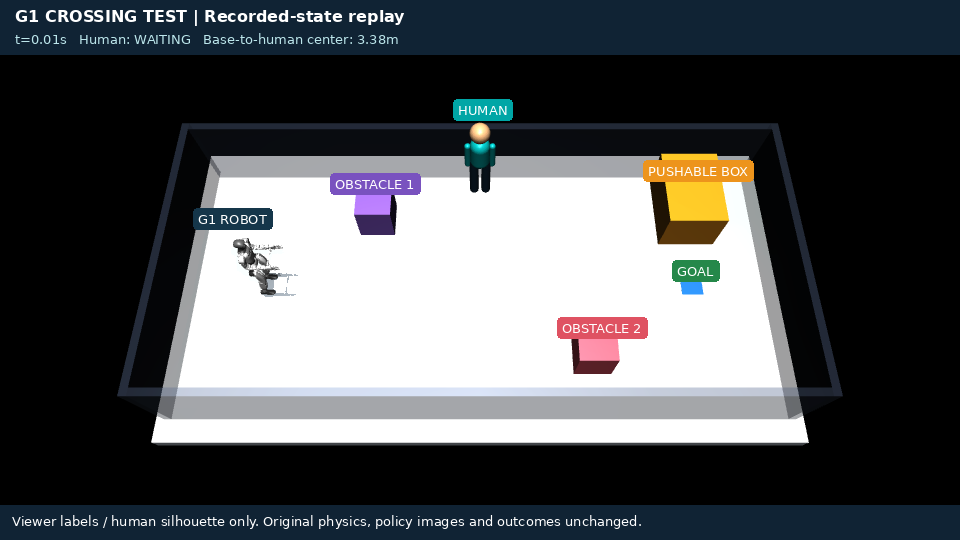
\includegraphics[width=0.42\textwidth,valign=c]{figures/humanoid_scene.png}\hfill
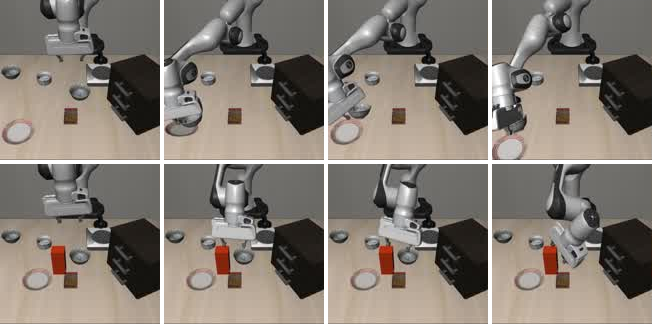
\includegraphics[width=0.56\textwidth,valign=c,trim=0 164 0 0,clip]{figures/arm_failure_frames.png}
\caption{실험 환경. (좌) G1 휴머노이드 횡단 장면: 장애물 2개, 밀 수 있는 상자, 목표, 이동하는 사람.
(우) LIBERO 로봇팔 장면: 테이블 중앙의 검은 그릇을 접시 위로 옮기는 과제.}\label{fig:env}
\end{figure*}

\begin{table*}[!t]
\centering\small
\caption{두 실험의 주요 조건 (세부 설정은 부록 A)}\label{tab:setup}
\begin{tabularx}{\textwidth}{@{}p{28mm}YY@{}}
\toprule
항목 & 실험 1: 로봇팔 pick-and-place & 실험 2: 휴머노이드 이동 \\
\midrule
로봇·정책 & LIBERO~\cite{libero}의 Franka Panda~\cite{panda} + GR00T~N1.7 (VLA)~\cite{groot,grootrepo} & Unitree G1~\cite{g1} + LLM Agent·경로 계획·GR00T 보행 제어~\cite{wbc} \\
작업 & 검은 그릇을 집어 접시에 놓기 & 상자·장애물·횡단하는 사람이 있는 통로에서 목표 도달 \\
환경 축 & 10 (그릇·접시 XY, 장애물 위치·크기·높이·회전) & 21 (물성, 통로 폭, 장애물 2개, 상자, 사람) \\
반복·예산 & 난수 시드 3개 $\times$ 방법별 4회 = 방법별 12회 & 난수 시드 1개, 방법별 유효 5회 \\
초기 장면 & 시드별 처음 2회는 양 방법 공통 무작위 장면 & 양 방법 공통 기준 장면 1회 \\
탐색 LLM & GPT-6 Luna Pro~\cite{luna}, 제안 6회 & GPT-6 Luna Pro~\cite{luna}, 제안 4회 \\
\bottomrule
\end{tabularx}
\end{table*}

그림~\ref{fig:env}는 두 실험의 환경이고, 표~\ref{tab:setup}은 주요 조건이다. 두 실험 모두 AFS와 Random은 같은 로봇, 작업, 성공 판정, 환경 변경 범위, 시도 예산을 사용한다.
AFS는 같은 시드 안의 자기 실행 이력만 참고하며, 다른 방법이나 과거 실험의 결과를 가져오지 않는다.

% ================================================================== 6
\section{실험 결과}

\subsection*{실패 발견율과 Random 대비 향상}
\begin{table}[!t]
\centering\footnotesize\setlength{\tabcolsep}{3pt}
\caption{AFS와 Random의 실패 발견 결과}\label{tab:result}
\begin{tabularx}{\linewidth}{@{}Ycccc@{}}
\toprule
& \multicolumn{2}{c}{실험 1: 로봇팔} & \multicolumn{2}{c}{실험 2: 휴머노이드} \\
\cmidrule(lr){2-3}\cmidrule(lr){4-5}
& AFS & Random & AFS & Random \\
\midrule
유효 시도 & 12 & 12 & 5 & 5 \\
PASS / FAIL & 5 / 7 & 10 / 2 & 3 / 2 & 5 / 0 \\
\textbf{실패 발견율 (FDR)} & \textbf{58.3\%} & 16.7\% & \textbf{40.0\%} & 0.0\% \\
탐색 단계 FDR (초기 장면 제외) & 6/6 (100\%) & 1/6 (16.7\%) & 2/4 (50\%) & 0/4 (0\%) \\
실패한 고유 환경 수 & 4 & 2 & 2 & 0 \\
\bottomrule
\end{tabularx}
\end{table}

\begin{figure}[!t]
\centering
\begin{tikzpicture}
\begin{axis}[
  ybar, width=\linewidth, height=48mm, bar width=9pt,
  ymin=0, ymax=125, ylabel={FDR (\%)}, ylabel style={font=\small},
  symbolic x coords={A,B,C,D}, xtick=data,
  xticklabels={{로봇팔\\전체},{로봇팔\\탐색 단계},{휴머노이드\\전체},{휴머노이드\\탐색 단계}},
  xticklabel style={font=\scriptsize,align=center},
  tick label style={font=\scriptsize},
  nodes near coords, nodes near coords style={font=\scriptsize},
  legend style={font=\scriptsize,at={(0.5,1)},anchor=north,draw=none,legend columns=2},
  axis lines*=left, enlarge x limits=0.18]
\addplot[fill=afs,draw=afs] coordinates {(A,58.3) (B,100) (C,40) (D,50)};
\addplot[fill=rnd,draw=rnd] coordinates {(A,16.7) (B,16.7) (C,0) (D,0)};
\legend{AFS, Random}
\end{axis}
\end{tikzpicture}
\caption{방법별 실패 발견율. 탐색 단계는 공통 초기 장면을 제외한 적응적 선택 구간이다.}\label{fig:fdr}
\end{figure}

표~\ref{tab:result}와 그림~\ref{fig:fdr}에 결과를 정리하였다. 로봇팔 실험에서 AFS의 FDR은 58.3\%로 목표 30\%를 넘었고, Random(16.7\%) 대비 상대 향상률은
$(58.3-16.7)/16.7 = 250\%$로 목표 20\%를 크게 웃돈다. 공통 초기 장면을 제외한 탐색 단계만 보면
AFS는 6회 모두 실패를 찾았고 Random은 1회였다. 시드별로도 AFS는 3/2/2건, Random은 1/1/0건으로
모든 시드에서 AFS가 더 많은 실패를 발견했다. 휴머노이드 실험에서도 AFS는 40\%, Random은 0\%로
40퍼센트포인트 차이를 보였다. 사람 안전 이벤트는 AFS 4/5회에서 검출되었다.

\subsection*{실패 유형 다양성}
\begin{table*}[!t]
\centering\small
\caption{초기 정의 6종 기준 실패 유형 발견 현황}\label{tab:div}
\begin{tabularx}{\textwidth}{@{}p{24mm}cp{26mm}Y@{}}
\toprule
유형 & 발견 & 실험 & 관측 근거 \\
\midrule
충돌 & \checkmark & 로봇팔 & 로봇–장애물 접촉 10.7--13.7초, 최대 접촉력 약 200--280\,N, 그릇 이동 1\,mm 미만 \\
장애물 간섭 & \checkmark & 휴머노이드 & 장애물 부근에서 경로 계획이 반복 거절되며 정체 \\
목표 위치 점유 & \checkmark & 휴머노이드 & 상자가 목표 영역을 점유, 목표 0.86\,m 앞에서 정체 \\
작업자 안전 위험 & \checkmark & 휴머노이드 & 사람과 1\,m 이내 0.5초 이상 노출 또는 접촉, AFS 4/5회 \\
도달 불가 & 후보 & 로봇팔·휴머노이드 & 그릇을 들어 운반했으나 접시 8.7\,cm 앞에서 미완료, 최종 목표점 경로 계획 반복 거절 \\
인식 오류 & -- & -- & 가림·유사 물체 조건은 후속 실험 \\
\midrule
\multicolumn{4}{@{}l}{\textbf{합계: 6종 중 4종 발견 + 도달 불가 후보 1종 (목표 4종 달성)}} \\
\bottomrule
\end{tabularx}
\end{table*}
표~\ref{tab:div}는 초기 정의 6종 기준의 발견 현황이다. 작업자 안전 위험은 목표 달성 여부와 무관하게 안전 요구사항을 위반한 실행을 실패 사례로 본다.
실제 실행에서는 초기 6종으로 설명하기 어려운 행동 실패도 관측되어, 넘어짐·이동 정체·물체 조작
실패·목표 완료 실패와 시스템 연동 문제 2종(최종 목표점 경로 계획 거절, 중간 목표 반복 도착)을 더한 12종 체계로 확장하였다(부록 B).
이 확장 체계로는 목표 완료 실패, 물체 조작 실패, 중간 목표 반복을 추가로 관측하였다.

% ================================================================== 7
\section{실패 사례 분석}

\begin{figure*}[!t]
\centering
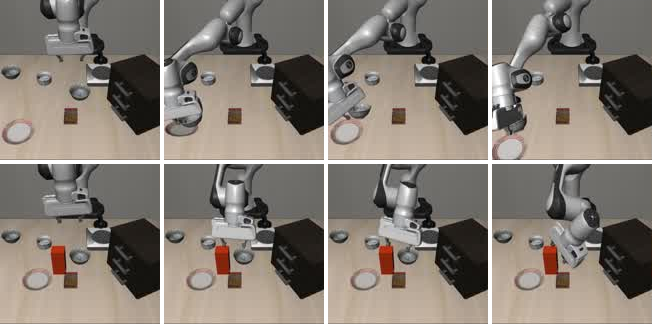
\includegraphics[width=0.72\textwidth]{figures/arm_failure_frames.png}
\caption{로봇팔 실패 사례(0, 2, 4, 7초). (위) 접시를 멀리 둔 장면: 그릇을 들어 운반하지만 접시 위에 놓지 못함.
(아래) 높이 15\,cm 장애물 장면: 그리퍼가 장애물에 걸려 그릇에 접근하지 못함.}\label{fig:arm}
\end{figure*}

\subsection*{로봇팔: 접근 차단 충돌과 PASS/FAIL 경계}
그림~\ref{fig:arm}은 대표 실패 장면이다. 실험 1의 FAIL 7건은 모두 제한 시간(약 15초) 안에 성공하지 못했고, 그릇은 전혀 들리지 않았으며
로봇과 장애물의 접촉이 10--14초 지속되었다. 반면 PASS는 약 5초 만에 끝나며 그릇이 15--17\,cm
들렸다가 접시 중심 2\,cm 이내에 놓였다. 즉 실패는 운반 중 충돌이 아니라 \textbf{잡기 전 접근 단계의
충돌}이다. AFS는 첫 실패의 접촉 기록을 읽고 장애물을 이송 경로 중앙에 크게 배치하는 방향으로
수렴하였다.

같은 정책으로 장애물 높이와 목표 거리를 단계적으로 바꾼 통제 실험(11개 장면)에서 명확한
경계가 확인되었다. 장애물 높이 10·12\,cm에서는 PASS, 14·15·17\,cm에서는 모두 FAIL이었고
최대 접촉력은 198--279\,N이었다. 접시를 기존 위치에서 이동 경로의 37.5\%까지 옮기면 PASS,
50\%에서는 그릇을 들고 운반했지만 접시 8.7\,cm 앞에서 놓지 못해 FAIL이었다.
따라서 이 정책의 안전 운용 경계는 \textbf{장애물 높이 12--14\,cm}, \textbf{목표 이동 37.5--50\%} 구간에 있다.

\subsection*{휴머노이드: 목표 위치 점유}
기준 장면 PASS(최종 목표 거리 0.116\,m) 뒤, AFS는 상자의 횡방향 위치만 1.0에서 0.0으로 바꿨다.
상자가 목표 영역을 점유하자 경로 계획기는 목표점이 막혀 있다며 목표 접근 요청을 거절했고,
상자 밀기 요청은 로봇이 상자 면과 약 90도 어긋난 방향에 있어 실행 전에 거절되었다.
로봇은 목표 0.86\,m 앞에서 허용된 행동 결정 10회를 모두 소진하였다. 두 축(상자 횡·종방향)을 바꾼
다른 FAIL에서도 목표점 거절과 우회 경로 차단이 반복되어 목표 0.43\,m 앞에서 종료되었다.
두 사례 모두 단순한 환경 변화가 경로 계획과 물체 밀기 기능의 한계를 드러낸 경우다.

% ================================================================== 8
\section{실패 자산화와 회귀 테스트}
탐색에서 찾은 실패는 한 번의 영상으로 끝나지 않고 재검증 가능한 테스트 자산이 되어야 한다.
모든 실행은 장면 파라미터, 시뮬레이션 모델, 작업 목표, 모델·소프트웨어 버전, 영상, 상태·접촉 기록,
기능 호출 결과를 위·변조 확인 정보와 함께 저장한다. 회귀 실행기는 이 기록을 읽어 동일
조건의 사례를 구성하고, 현재 버전으로 고정 예산 안에서 재실행한 뒤 원본과 비교한다.

\begin{enumerate}
\item 저장된 PASS/FAIL 사례를 읽고 동일 조건·장면의 사례를 묶는다.
\item 사례별 반복 수와 호출 상한을 정하고 입력·자산 호환성을 검사한다.
\item 현재 버전 조건을 기록한 뒤 재실행한다.
\item 원본과 신규 결과를 유지, 퇴행, 개선, 혼재 등으로 분류하고 영상·근거가 연결된 보고서를 생성한다(부록 E).
\end{enumerate}

정상 완료 사례도 함께 유지해 정책 업데이트 후 기존 성공이 깨지는지 확인한다. 본 과제에서 발견한
장애물 높이 경계(12/14\,cm)와 목표 점유 장면은 정책이나 현장 배치가 바뀔 때 우선 재실행할
회귀 테스트셋의 핵심 사례가 된다.

% ================================================================== 9
\section{결론}
표~\ref{tab:goal}에 목표 달성 현황을 정리하였다.

\begin{table*}[!t]
\centering\small
\caption{목표 달성 현황}\label{tab:goal}
\begin{tabularx}{\textwidth}{@{}p{40mm}p{28mm}Y@{}}
\toprule
목표 & 결과 & 근거 \\
\midrule
실패 발견율 30\% 이상 & \textbf{달성} & 로봇팔 58.3\%, 휴머노이드 40\% \\
Random 대비 20\% 이상 향상 & \textbf{달성} & 로봇팔 상대 250\% (16.7\%$\to$58.3\%), 휴머노이드 +40\%p \\
실패 유형 6종 중 4종 & \textbf{달성} & 충돌, 장애물 간섭, 목표 위치 점유, 작업자 안전 위험 + 도달 불가 후보 \\
3D 장면 구조화·후보 생성 & 구현 & 10축·21축 환경 변경, 장면 그래프·시뮬레이션 모델 생성, 실행 전 검사 \\
행동 기반 취약 조건 탐색 & 구현 & 관측$\to$가설$\to$제안$\to$FAIL 연결 확인 \\
회귀 테스트 자산화 & 구현 & 실행 기록 저장, 재실행·비교 실행기 \\
\bottomrule
\end{tabularx}
\end{table*}

본 과제는 3D 장면 파라미터화, LLM 기반 능동 실패 탐색, 단계적 판정, 회귀 자산화를 하나의
파이프라인으로 구현하였다. VLA 기반 로봇팔에서 AFS는 같은 예산으로 Random보다 3.5배 많은 실패를
찾았고, 휴머노이드에서도 Random이 찾지 못한 실패를 발견했다. 또한 장애물 높이와 목표 거리에 대한
PASS/FAIL 경계를 정량적으로 제시하여, 배포 전 검증에서 어떤 조건을 우선 점검해야 하는지 알려준다.

현재 실험은 시드 수와 반복 수가 작고, AFS가 동일 환경을 반복 제안하는 경향이 있다.
후속 과제로 (1) 더 많은 시드에서의 독립 평가, (2) 새로운 환경 탐색을 보상하는 다양성 목표,
(3) 유사 물체·카메라 가림 조건을 통한 인식 오류 탐색, (4) 선정 사례의 실제 회귀 재실행을 진행한다.

% ================================================================== 참고문헌
\begin{thebibliography}{99}\small
\setlength{\itemsep}{0pt}
\bibitem{rt2} A. Brohan et al., ``RT-2: Vision-Language-Action Models Transfer Web Knowledge to Robotic Control,'' \textit{Conference on Robot Learning (CoRL)}, 2023.
\bibitem{corso} A. Corso, R. Moss, M. Koren, R. Lee, M. Kochenderfer, ``A Survey of Algorithms for Black-Box Safety Validation of Cyber-Physical Systems,'' \textit{Journal of Artificial Intelligence Research}, vol.~72, 2021.
\bibitem{ast} R. Lee, M. Kochenderfer, O. Mengshoel, G. Brat, M. Owen, ``Adaptive Stress Testing of Airborne Collision Avoidance Systems,'' \textit{IEEE/AIAA Digital Avionics Systems Conference}, 2015.
\bibitem{robosuite} Y. Zhu, J. Wong, A. Mandlekar, R. Mart\'{i}n-Mart\'{i}n et al., ``robosuite: A Modular Simulation Framework and Benchmark for Robot Learning,'' arXiv:2009.12293, 2020.
\bibitem{libero} B. Liu, Y. Zhu, C. Gao, Y. Feng, Q. Liu, Y. Zhu, P. Stone, ``LIBERO: Benchmarking Knowledge Transfer for Lifelong Robot Learning,'' \textit{NeurIPS Datasets and Benchmarks}, 2023. \url{https://github.com/Lifelong-Robot-Learning/LIBERO}
\bibitem{groot} NVIDIA, ``GR00T N1: An Open Foundation Model for Generalist Humanoid Robots,'' arXiv:2503.14734, 2025.
\bibitem{mujoco} E. Todorov, T. Erez, Y. Tassa, ``MuJoCo: A Physics Engine for Model-Based Control,'' \textit{IEEE/RSJ IROS}, 2012.
\bibitem{sg} I. Armeni, Z.-Y. He, J. Gwak, A. Zamir, M. Fischer, J. Malik, S. Savarese, ``3D Scene Graph: A Structure for Unified Semantics, 3D Space, and Camera,'' \textit{ICCV}, 2019.
\bibitem{mjcf} Google DeepMind, ``MuJoCo Documentation: XML Reference (MJCF),'' \url{https://mujoco.readthedocs.io/en/stable/XMLreference.html}.
\bibitem{panda} S. Haddadin et al., ``The Franka Emika Robot: A Reference Platform for Robotics Research and Education,'' \textit{IEEE Robotics \& Automation Magazine}, vol.~29, no.~2, 2022.
\bibitem{grootrepo} NVIDIA, ``Isaac GR00T,'' \url{https://github.com/NVIDIA/Isaac-GR00T}; 모델 체크포인트 ``GR00T-N1.7-LIBERO,'' \url{https://huggingface.co/nvidia/GR00T-N1.7-LIBERO}.
\bibitem{g1} Unitree Robotics, ``Unitree G1 Humanoid Robot,'' \url{https://www.unitree.com/g1}.
\bibitem{wbc} NVIDIA, ``GR00T-WholeBodyControl,'' \url{https://github.com/NVlabs/GR00T-WholeBodyControl}.
\bibitem{luna} OpenRouter, ``OpenAI: GPT-6 Luna Pro,'' \url{https://openrouter.ai/openai/gpt-6-luna-pro}.
\end{thebibliography}

% ================================================================== 부록
\onecolumn
\appendix
\renewcommand{\thesection}{부록 \Alph{section}}
\renewcommand{\thetable}{\Alph{section}.\arabic{table}}
\setcounter{table}{0}

\section{실험 설정 상세}

\subsection*{A.1 실험 1: 로봇팔 pick-and-place}
\begin{table}[H]
\centering\small
\caption{로봇팔 실험 조건}
\begin{tabularx}{\linewidth}{@{}p{38mm}Y@{}}
\toprule
항목 & 값 \\
\midrule
시뮬레이터·과제 & LIBERO-Spatial~\cite{libero} (robosuite~\cite{robosuite}·MuJoCo~\cite{mujoco}), ``테이블 중앙의 검은 그릇을 집어 접시 위에 놓기'' \\
로봇 & Franka Emika Panda 7자유도 로봇팔 + 평행 그리퍼~\cite{panda} \\
정책 & NVIDIA GR00T~N1.7, LIBERO-Spatial용 공개 체크포인트~\cite{groot,grootrepo} \\
제어 & 실행당 최대 300 제어 단계(약 15초), 한 번의 추론으로 8단계 동작 생성 \\
성공 판정 & LIBERO 기본 성공 판정 (그릇이 접시 위에 놓임) \\
난수 시드 & 661, 673, 677 (방법별 시드당 4회, 처음 2회는 공통 무작위 초기 장면) \\
탐색 LLM & GPT-6 Luna Pro~\cite{luna}, 제안 상한 6회, 응답 제한 300초, 자동 재시도 없음 \\
배경 & 나머지 물체 배치는 모든 실행에서 동일, 방해용 검은 그릇 1개는 작업 영역 밖에 고정 \\
측정 & 로봇·그릇과 장애물의 접촉 시간과 접촉력, 그릇 낙하, 그릇–접시 거리 \\
총 제어 단계 & AFS 2,591, Random 1,590 \\
\bottomrule
\end{tabularx}
\end{table}

\begin{table}[H]
\centering\small
\caption{로봇팔 환경 변형 축 (테이블 작업공간 기준, 단위 m·rad)}
\begin{tabularx}{\linewidth}{@{}p{38mm}Y@{}}
\toprule
축 & 범위 \\
\midrule
그릇 X / Y & $[-0.10, -0.05]$ / $[-0.01, 0.01]$ \\
접시 X / Y & $[0.06, 0.10]$ / $[0.19, 0.24]$ \\
장애물 X / Y & $[-0.24, -0.0075]$ / $[0.09, 0.12]$ \\
장애물 폭 / 깊이 / 높이 & $[0.02, 0.06]$ / $[0.02, 0.06]$ / $[0.02, 0.17]$ \\
장애물 회전 & $[-\pi/2, \pi/2]$ \\
\bottomrule
\end{tabularx}
\end{table}

\subsection*{A.2 실험 2: 휴머노이드 이동}
\begin{table}[H]
\centering\small
\caption{휴머노이드 실험 조건}
\begin{tabularx}{\linewidth}{@{}p{38mm}Y@{}}
\toprule
항목 & 값 \\
\midrule
장면 & 사람이 통로를 가로지르는 이동 장면, 21개 변경 축 \\
로봇 & Unitree G1 29자유도 모델~\cite{g1}, MuJoCo~\cite{mujoco} 시뮬레이션 \\
제어 구조 & 상위 LLM Agent + 경로 계획·추종 + GR00T 보행 정책~\cite{wbc} \\
로봇·AFS 모델 & 모두 GPT-6 Luna Pro~\cite{luna} \\
목표 판정 & 목표 반경 0.25\,m 안에서 1초 이상 체류, 상자 밀기 허용 \\
반복·예산 & 난수 시드 1개, 방법별 유효 5회(시도 상한 7회), 실행당 로봇 행동 결정 상한 10회, AFS 제안 상한 6회 \\
변경 규칙 & 공통 기준 장면에서 1개·2개 축 변경을 교대 배정, 최소 변경량은 축 범위의 10\%, 매번 기준 장면에서 새로 변경 \\
사람 안전 측정 & 로봇과 사람 사이 1\,m 이내에 0.5초 이상 머물거나 접촉하면 안전 이벤트 \\
\bottomrule
\end{tabularx}
\end{table}

\begin{table}[H]
\centering\small
\caption{휴머노이드 환경 변형 축}
\begin{tabularx}{\linewidth}{@{}p{34mm}cY@{}}
\toprule
환경 요소 & 축 수 & 변형 내용 및 범위 \\
\midrule
물체·바닥 물성 & 3 & 상자 질량 0.2--10\,kg, 상자·바닥 마찰계수 0.05--1.5 \\
통로와 상자 배치 & 2 & 통로 폭 1.6--4.0\,m, 상자 횡방향 위치 비율 \\
장애물 형상·배치 & 12 & 장애물 2개 각각의 종·횡방향 위치, 가로·세로 크기, 높이, 회전 \\
목표 부근 상자 위치 & 1 & 상자 종방향 위치 6.8--7.5\,m \\
사람 이동 & 3 & 종방향 위치 3.65--4.35\,m, 속도 0.1--1.5\,m/s, 출발 거리 0.5--5\,m \\
\midrule
합계 & 21 & \\
\bottomrule
\end{tabularx}
\end{table}

\section{실패 유형 판정 규칙}
\begin{table}[H]
\centering\small
\caption{12종 실패 유형 체계}
\begin{tabularx}{\linewidth}{@{}p{24mm}p{32mm}Y@{}}
\toprule
분류 & 유형 & 판정 규칙 (요약) \\
\midrule
\multirow{6}{24mm}{초기 환경·물리 6종} & 충돌 & 로봇 몸체와 장애물의 접촉이 지속되며 작업 실패 \\
& 도달 불가 & 목표점 계획이 반복 거절되거나, 물체 운반 후 목표 위치 미완료 \\
& 장애물 간섭 & 마지막 10초에 경로 계획 거절 2회 이상, 장애물과 0.55\,m 이내, 정체 \\
& 목표 위치 점유 & 목표 영역이 물체로 점유된 상태에서 종료 구간 정체 \\
& 작업자 안전 위험 & 사람과 접촉 또는 1\,m 이내 0.5초 이상 연속 노출 \\
& 인식 오류 & 잘못된 대상 선택, 가림에 의한 인식 실패 \\
\midrule
\multirow{4}{24mm}{행동 수행 4종} & 넘어짐 & 몸통 높이 0.45\,m 미만 또는 기울기 60도 이상이 0.5초 이상 \\
& 이동 정체 & 2초 이상의 이동 실행에서 순이동 0.05\,m 이하 \\
& 물체 조작 실패 & 상자 밀기 등 조작 요청이 최종적으로 거절·실패 \\
& 목표 완료 실패 & 목표 반경 안에 도착했으나 체류 시간 미충족 \\
\midrule
\multirow{2}{24mm}{시스템 관측 2종} & 최종 목표점 계획 거절 & 경로 계획기가 최종 목표점을 막힘으로 2회 이상 거절, 마지막 행동도 거절 \\
& 중간 목표 반복 & 최종 목표 밖 같은 중간 목표에 반복 도착 \\
\bottomrule
\end{tabularx}
\end{table}
한 실행에서 여러 현상이 관측되면 대표 유형 1개만 집계하고 나머지는 보조 진단으로 보존한다.
상태 기록 간격이 0.25초를 넘거나 필수 기록이 없으면 판정을 보류한다.

\section{AFS 제안과 피드백}
\begin{table}[H]
\centering\small
\caption{AFS에 제공하는 행동 관측}
\begin{tabularx}{\linewidth}{@{}p{38mm}Y@{}}
\toprule
관측 정보 & 활용 \\
\midrule
목표점 경로 거절·반복 & 같은 지점에 대한 거절 반복 파악 \\
중간 목표 도착 & 부분 이동 성공과 전체 과제 완료의 차이 파악 \\
목표 거리 변화·최종 상태 & 실제 진전과 종료 상태 구분 \\
조작 요청과 그 결과 & 요청과 실제 물리 실행의 구분 \\
접촉 시간·물체 이동량 (로봇팔) & 접근 차단과 운반·놓기 실패의 구분 \\
예상 유형과 측정 유형 & 예상이 실제 검출로 이어졌는지 확인 \\
\bottomrule
\end{tabularx}
\end{table}

\textbf{제안 예시 (로봇팔, 시드 661, 탐색 1회차).} 가설: ``그릇에서 접시로 옮기는 경로 중앙에
더 크고 높은 상자를 두면 로봇의 움직임이 막혀 그릇을 옮기지 못할 것이다.''
제안값: 그릇 (-0.080, 0.007), 접시 (0.084, 0.239), 장애물 위치 (-0.041, 0.118), 폭·깊이 0.06\,m,
높이 0.17\,m, 회전 0. 결과: FAIL, 로봇–장애물 접촉 11.0초.

\section{시도별 결과}
\begin{table}[H]
\centering\scriptsize
\caption{로봇팔 실험 시도별 결과 (b: 공통 초기 장면, s: 탐색 단계)}
\begin{tabular}{@{}lccccc|ccccc@{}}
\toprule
& \multicolumn{5}{c|}{AFS} & \multicolumn{5}{c}{Random} \\
시드 / 순번 & 단계 & 결과 & 제어 단계 & 접촉(s) & 그릇–접시(m) & 단계 & 결과 & 제어 단계 & 접촉(s) & 그릇–접시(m) \\
\midrule
661 / 0 & b & FAIL & 300 & 13.33 & 0.284 & b & FAIL & 300 & 13.33 & 0.284 \\
661 / 1 & b & PASS & 96 & 0.00 & 0.021 & b & PASS & 96 & 0.00 & 0.021 \\
661 / 2 & s & FAIL & 300 & 11.04 & 0.284 & s & PASS & 95 & 0.00 & 0.007 \\
661 / 3 & s & FAIL & 300 & 10.73 & 0.284 & s & PASS & 102 & 0.00 & 0.011 \\
673 / 0 & b & PASS & 103 & 0.02 & 0.019 & b & PASS & 103 & 0.02 & 0.019 \\
673 / 1 & b & PASS & 98 & 0.00 & 0.008 & b & PASS & 98 & 0.00 & 0.008 \\
673 / 2 & s & FAIL & 300 & 12.79 & 0.275 & s & FAIL & 300 & 13.24 & 0.254 \\
673 / 3 & s & FAIL & 300 & 12.45 & 0.275 & s & PASS & 102 & 0.00 & 0.013 \\
677 / 0 & b & PASS & 95 & 0.23 & 0.019 & b & PASS & 95 & 0.23 & 0.019 \\
677 / 1 & b & PASS & 99 & 0.13 & 0.004 & b & PASS & 99 & 0.13 & 0.004 \\
677 / 2 & s & FAIL & 300 & 13.73 & 0.312 & s & PASS & 100 & 0.00 & 0.014 \\
677 / 3 & s & FAIL & 300 & 13.74 & 0.312 & s & PASS & 100 & 0.00 & 0.009 \\
\bottomrule
\end{tabular}
\end{table}

\begin{table}[H]
\centering\small
\caption{로봇팔 통제 실험 (장애물 높이·목표 거리 경계)}
\begin{tabularx}{\linewidth}{@{}Ycccc@{}}
\toprule
장면 & 결과 & 제어 단계 & 장애물 접촉(s) & 최종 그릇–접시(m) \\
\midrule
목표 이동 0 / 12.5 / 25\% & PASS & 103 / 98 / 95 & 0 & 0.015 / 0.016 / 0.018 \\
목표 이동 37.5\% & PASS & 261 & 0 & 0.030 \\
목표 이동 50\% & FAIL & 300 & 0 & 0.087 \\
장애물 높이 10 / 12\,cm & PASS & 97 / 98 & 0 & 0.006 / 0.008 \\
장애물 높이 14 / 15 / 17\,cm & FAIL & 300 & 13.5--13.6 & 0.241 \\
높이 15\,cm, 왼쪽 3\,cm 이동 & FAIL & 300 & 13.5 & 0.241 \\
\bottomrule
\end{tabularx}
\end{table}

\begin{table}[H]
\centering\small
\caption{휴머노이드 실험 집계와 비용}
\begin{tabularx}{\linewidth}{@{}Yrr@{}}
\toprule
& AFS & Random \\
\midrule
시도 / 유효 / 제외 & 5 / 5 / 0 & 6 / 5 / 1 \\
PASS / FAIL & 3 / 2 & 5 / 0 \\
AFS 제안 / 로봇 행동 결정 & 4 / 39 & 0 / 27 \\
사람 안전 이벤트 (목표 PASS와 동반) & 4/5 (2) & 5/5 (5) \\
로봇 입력 / 출력 토큰 & 3,683,079 / 253,986 & 1,675,999 / 185,937 \\
AFS 제안 입력 / 출력 토큰 & 689,414 / 53,475 & -- \\
\bottomrule
\end{tabularx}
\end{table}
Random의 제외 1회는 LLM 응답이 제한 시간을 넘겨 판정 불가로 처리했으며, 재실행 없이 다음 순서를 진행했다.
휴머노이드 영상은 12\,fps 실시간 기록이며, 실행 시간의 82--92\%는 LLM 추론 대기(위치·자세 유지) 구간이다.

\section{회귀 테스트 비교 상태}
\begin{table}[H]
\centering\small
\caption{회귀 비교 상태 정의}
\begin{tabularx}{\linewidth}{@{}p{52mm}Y@{}}
\toprule
상태 & 의미 \\
\midrule
유지 (성공 / 실패) & 이전과 같은 목표 결과 \\
퇴행 & 이전에 성공한 사례가 새 버전에서 실패 \\
개선 & 이전에 실패한 사례가 새 버전에서 성공 \\
혼재 & 이전 또는 새 반복에서 성공과 실패가 섞임 \\
대기 / 판정 불가 & 미완료 또는 제외로 비교 불가 \\
\bottomrule
\end{tabularx}
\end{table}

\section{용어와 사용 도구}
\subsection*{F.1 시뮬레이션과 장면 표현}
\begin{table}[H]
\centering\small
\caption{시뮬레이션·장면 표현 관련 도구}
\begin{tabularx}{\linewidth}{@{}p{30mm}Y@{}}
\toprule
용어 & 설명과 본 과제에서의 역할 \\
\midrule
MuJoCo~\cite{mujoco} & 접촉이 많은 로봇 동작을 빠르고 정확하게 계산하는 물리 엔진이다. 현재 Google DeepMind가 오픈소스로 관리한다. 두 실험 모두 로봇·물체·장애물의 움직임과 접촉을 MuJoCo로 계산했다. \\
MJCF (MuJoCo XML)~\cite{mjcf} & MuJoCo가 읽는 XML 형식의 모델 파일이다. 물체(body), 관절(joint), 충돌 형상(geom), 구동기(actuator), 마찰·질량 같은 물성을 기술한다. 환경 생성기는 장면 파라미터가 바뀔 때마다 이 파일을 새로 만들어 장애물의 위치·크기·회전과 물성을 반영한다. \\
3D 장면 그래프~\cite{sg} & 장면의 객체를 노드, 객체 사이의 공간 관계(거리, 인접, 점유 등)를 간선으로 나타낸 그래프다. 본 과제에서는 객체의 위치·크기·역할과 목표 영역 점유 여부를 구조화하여, 생성된 시뮬레이션 모델과 이동 지도가 서로 일치하는지 검사하는 기준으로 사용했다. \\
이동 지도 & 휴머노이드의 경로 계획에 쓰는 2차원 격자 지도다. 장애물과 상자가 차지하는 영역을 표시하며, 장면 그래프와 같은 파라미터에서 생성된다. \\
robosuite~\cite{robosuite} & MuJoCo 위에서 로봇팔 조작 환경을 구성하는 시뮬레이션 프레임워크다. LIBERO가 이를 기반으로 만들어졌다. \\
\bottomrule
\end{tabularx}
\end{table}

\subsection*{F.2 로봇과 정책}
\begin{table}[H]
\centering\small
\caption{로봇·정책 관련 도구}
\begin{tabularx}{\linewidth}{@{}p{30mm}Y@{}}
\toprule
용어 & 설명과 본 과제에서의 역할 \\
\midrule
VLA~\cite{rt2} & Vision-Language-Action 모델. 카메라 영상과 자연어 명령을 입력받아 로봇의 관절·그리퍼 동작을 직접 출력하는 신경망 정책이다. 실험 1의 로봇팔 정책이 이에 해당한다. \\
LIBERO~\cite{libero} & 언어 명령 기반 로봇팔 조작 벤치마크로, 130개 과제가 Spatial·Object·Goal·Long 등의 묶음으로 구성된다. 본 과제는 같은 물체를 서로 다른 배치에 두고 ``그릇을 접시에 놓기''를 수행하는 LIBERO-Spatial의 과제 하나를 사용했고, 성공 여부는 LIBERO의 기본 판정을 그대로 따랐다. \\
Franka Emika Panda~\cite{panda} & 연구용으로 널리 쓰이는 7자유도 로봇팔이다. LIBERO 환경의 기본 로봇이며, 실험 1에서 평행 그리퍼로 그릇을 집는다. \\
GR00T~N1 / N1.7~\cite{groot,grootrepo} & NVIDIA가 공개한 로봇용 VLA 기반 모델이다. 영상과 언어를 이해하는 시각-언어 모듈과 연속 동작을 생성하는 동작 생성 모듈로 구성된다. 본 과제는 학습이나 수정 없이 N1.7 버전의 LIBERO-Spatial용 공개 체크포인트를 그대로 사용했다. 한 번의 추론으로 8단계 분량의 동작을 출력한다. \\
Unitree G1~\cite{g1} & Unitree사의 키 약 1.3\,m 휴머노이드 로봇이다. 실험 2에서는 29자유도 시뮬레이션 모델을 사용했다. \\
GR00T 보행 정책~\cite{wbc} & NVIDIA가 공개한 G1용 학습 기반 보행·균형 제어기다. 상위 계층이 정한 이동 속도와 방향을 관절 명령으로 바꿔 넘어지지 않고 걷게 한다. 본 과제에서는 학습 없이 그대로 사용했다. \\
LLM Agent (휴머노이드) & 실험 2의 상위 의사결정기다. 로봇 카메라 영상과 목표를 보고 경로 계획, 목표점 이동, 직접 이동, 상자 밀기 같은 로봇 기능 중 하나를 골라 호출한다. 한 번의 선택을 ``행동 결정''이라 하며 실행당 10회로 제한했다. \\
\bottomrule
\end{tabularx}
\end{table}

\subsection*{F.3 탐색·평가 용어}
\begin{table}[H]
\centering\small
\caption{탐색·평가 관련 용어}
\begin{tabularx}{\linewidth}{@{}p{30mm}Y@{}}
\toprule
용어 & 설명 \\
\midrule
GPT-6 Luna Pro~\cite{luna} & OpenAI의 대형 언어 모델로, OpenRouter API를 통해 호출했다. 실험 1·2의 AFS 탐색기와 실험 2의 로봇 LLM Agent에 사용했다. \\
AFS & Active Failure Search. 이전 실행 결과를 근거로 실패 가능성이 높은 다음 테스트 환경을 골라 실행하는 능동 탐색 방법이다. 본 과제에서는 LLM이 가설과 환경 변경값을 제안하고, 별도 검증기가 범위와 예산을 확인한다. \\
Random & 비교 기준 방법. 같은 허용 범위에서 환경 변경 축과 값을 균등하게 무작위로 뽑으며, 이전 결과를 참고하지 않는다. \\
환경 변경 축 & 테스트 장면에서 바꿀 수 있는 하나의 수치 항목(예: 장애물 높이, 통로 폭)이다. 실험 1은 10개, 실험 2는 21개다. \\
FDR & Failure Discovery Rate. 판정 가능한 유효 실행 중 작업에 실패한 실행의 비율이다. \\
난수 시드 & 시뮬레이션과 무작위 추출의 난수 초깃값이다. 같은 시드에서는 두 방법이 같은 초기 조건으로 시작한다. \\
제어 단계 & 로봇 정책이 동작 명령을 한 번 내리는 시간 단위다. 실험 1에서는 1단계가 약 0.05초이며, 300단계(약 15초) 안에 과제를 끝내지 못하면 실패다. \\
초기 장면 / 탐색 단계 & 각 시드의 처음 실행은 두 방법이 같은 무작위 장면을 쓰는 초기 장면이고, 이후는 각 방법이 스스로 장면을 고르는 탐색 단계다. \\
회귀 테스트 & 정책이나 현장 조건이 바뀐 뒤, 이전에 저장한 성공·실패 사례를 다시 실행해 결과가 유지되는지 확인하는 테스트다. \\
\bottomrule
\end{tabularx}
\end{table}

\end{document}
